\section{Analysis}
\subsection{PCA eigenvectors}

We were successfully able to create a set of eigenvectors from the twenty-three supernovae. Using just three eigenvectors we are able to account for 91.3\% of
variation within the sample, and with five eigenvectors we account for 95.8\% of variation. 

%% The values (usually only l,r and c) in the last part of
%% \begin{deluxetable}{} command tell LaTeX how many columns
%% there are and how to align them.
\begin{deluxetable}{ccccccccc}

%% Keep a portrait orientation

%% Over-ride the default font size
%% Use Default (12pt)

%% Use \tablewidth{?pt} to over-ride the default table width.
%% If you are unhappy with the default look at the end of the
%% *.log file to see what the default was set at before adjusting
%% this value.

%% This is the title of the table.
\tablecaption{First Five Normalized Weights for Each Supernova}

%% This command over-rides LaTeX's natural table count
%% and replaces it with this number.  LaTeX will increment 
%% all other tables after this table based on this number
\tablenum{4}

%% The \tablehead gives provides the column headers.  It
%% is currently set up so that the column labels are on the
%% top line and the units surrounded by ()s are in the 
%% bottom line.  You may add more header information by writing
%% another line between these lines. For each column that requries
%% extra information be sure to include a \colhead{text} command
%% and remember to end any extra lines with \\ and include the 
%% correct number of &s.
\tablehead{\colhead{Supernova} & \colhead{Class} & \colhead{Radius} & \colhead{$\theta$} & \colhead{$\sigma_{1}$} & \colhead{$\sigma_{2}$} & \colhead{$\sigma_{3}$} & \colhead{$\sigma_{4}$} & \colhead{$\sigma_{5}$} \\ 
\colhead{} & \colhead{} & \colhead{} & \colhead{} & \colhead{} & \colhead{} & \colhead{} & \colhead{} & \colhead{} } 

%% All data must appear between the \startdata and \enddata commands
\startdata
SN1991bg & III & 2.21 & 214.53 & -1.82274 & -1.25405 & 2.32927 & -0.29614 & -1.70822 \\
SN1991T & IV & 2.31 & 280.47 & 0.41972 & -2.27191 & -0.15796 & -1.07779 & 0.64694 \\
SN1997dt & III & 1.16 & 182.43 & -1.15496 & -0.04904 & -0.82824 & -0.77541 & 0.52835 \\
SN1998aq & IV & 0.96 & 355.83 & 0.96126 & -0.07014 & 0.00158 & -1.12395 & -0.39967 \\
SN1998bp & II & 0.76 & 133.35 & -0.52207 & 0.55304 & 1.19854 & -0.32893 & 1.80270 \\
SN1998de & III & 1.52 & 192.12 & -1.48267 & -0.31837 & 1.94749 & 2.10701 & 0.44297 \\
SN1998dh & I & 1.38 & 83.33 & 0.16048 & 1.37175 & -0.32390 & 1.19359 & -0.10991 \\
SN1998ec & Zero & 0.33 & 143.09 & -0.26456 & 0.19873 & -1.02778 & 1.51962 & -0.65194 \\
SN1998eg & I & 1.25 & 55.73 & 0.70201 & 1.03018 & 0.34618 & -0.38230 & -0.43956 \\
SN1998es & IV & 0.78 & 309.59 & 0.49563 & -0.59931 & -0.26691 & -0.40891 & -0.86157 \\
SN1998V & Zero & 0.62 & 32.21 & 0.52586 & 0.33128 & -0.05399 & -0.24062 & -1.10653 \\
SN1999aa & IV & 1.19 & 327.14 & 0.99893 & -0.64514 & -0.31026 & -0.15829 & -0.73372 \\
SN1999ac & I & 0.99 & 60.95 & 0.48125 & 0.86625 & 0.46076 & 0.15119 & -1.02274 \\
SN1999cc & I & 1.02 & 67.86 & 0.38283 & 0.94092 & -0.71142 & 1.05519 & 0.89260 \\
SN1999cl & II & 2.73 & 178.91 & -2.72918 & 0.05201 & -2.43622 & -0.50893 & -0.23464 \\
SN1999dq & IV & 0.95 & 294.66 & 0.39755 & -0.86608 & -0.22107 & -0.20711 & -0.53821 \\
SN1999ej & Zero & 0.20 & 19.25 & 0.18974 & 0.06626 & -0.33475 & -0.46655 & 1.59778 \\
SN1999gd & II & 1.15 & 152.48 & -1.02299 & 0.53288 & -0.30726 & -1.34928 & 0.46196 \\
SN1999gp & IV & 1.11 & 321.67 & 0.86747 & -0.68577 & -0.40707 & 0.67967 & -0.47576 \\
SN2000cf & I & 1.41 & 57.20 & 0.76164 & 1.18204 & 1.04556 & -1.83399 & -0.07544 \\
SN2000cx & IV & 2.35 & 295.33 & 1.00485 & -2.12255 & -0.21715 & 1.13353 & 1.76569 \\
SN2000dk & I & 1.33 & 82.33 & 0.17780 & 1.32041 & 0.81927 & 0.04584 & 1.39704 \\
SN2000fa & Zero & 0.64 & 42.76 & 0.47216 & 0.43659 & -0.54467 & 1.27253 & -1.17814 \\
\enddata

%% Include any \tablenotetext{key}{text}, \tablerefs{ref list},
%% or \tablecomments{text} between the \enddata and 
%% \end{deluxetable} commands

%% No \tablecomments indicated

%% No \tablerefs indicated

\end{deluxetable}


\begin{figure}[htp]
\begin{center}
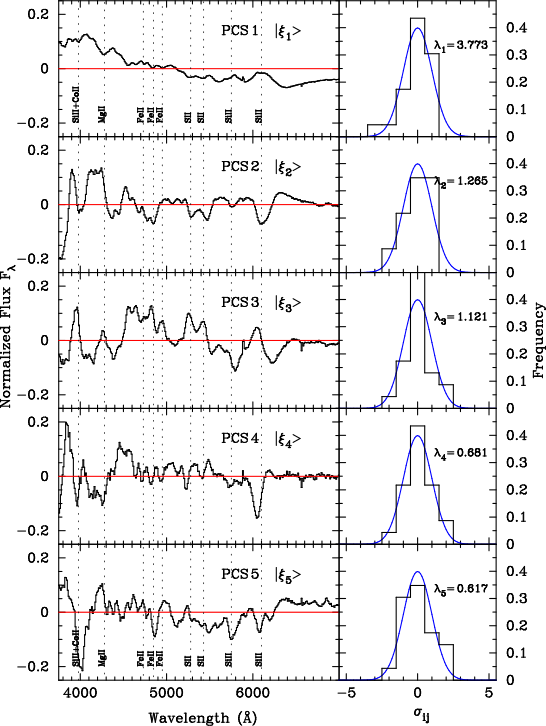
\includegraphics[angle=0,scale=0.8]{./figures/pca/20SNe_PCS_01to05_areanorm.ps}
%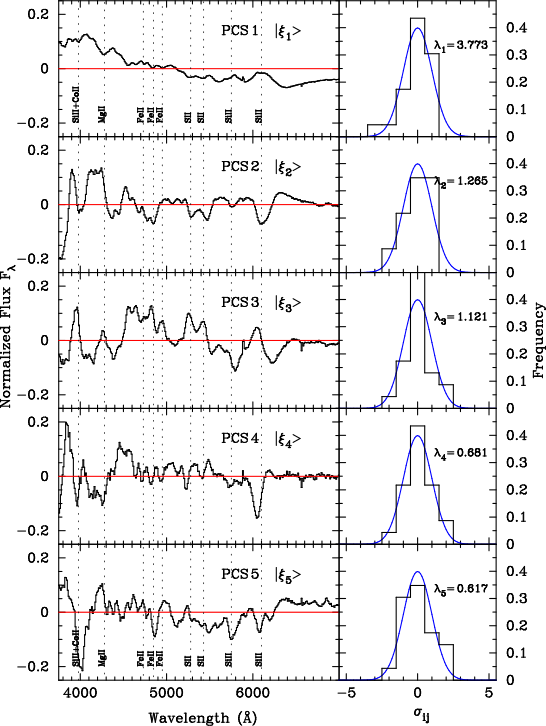
\includegraphics[angle=0,scale=0.4]{./figures/pca/20SNe_PCS_01to05_areanorm.ps}
%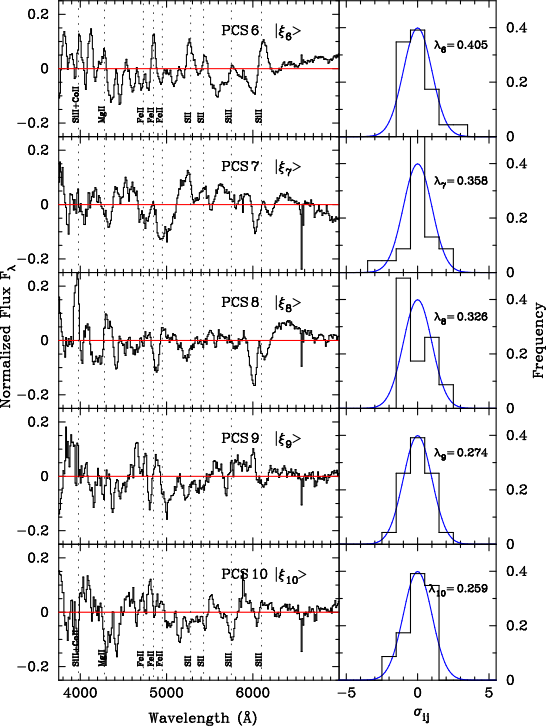
\includegraphics[angle=0,scale=0.4]{./figures/pca/20SNe_PCS_06to10_areanorm.ps}
\end{center}
\caption{
The first five eigenvectors, which account for 95.8\% of variation in the sample. Note the slope of the first eigenvector.
}
\label{fig:eigne1}
\end{figure}
\begin{figure}[htp]
\begin{center}
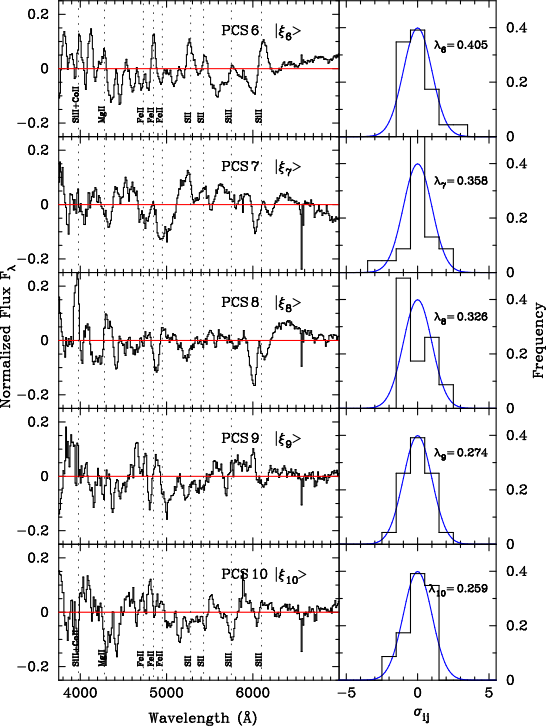
\includegraphics[angle=0,scale=0.8]{./figures/pca/20SNe_PCS_06to10_areanorm.ps}
\end{center}
\caption{
Eigenvectors six through ten, which account for 2.9\% of variation in the sample. 
}
\label{fig:eigen2}
\end{figure}
\begin{figure}[htp]
\begin{center}
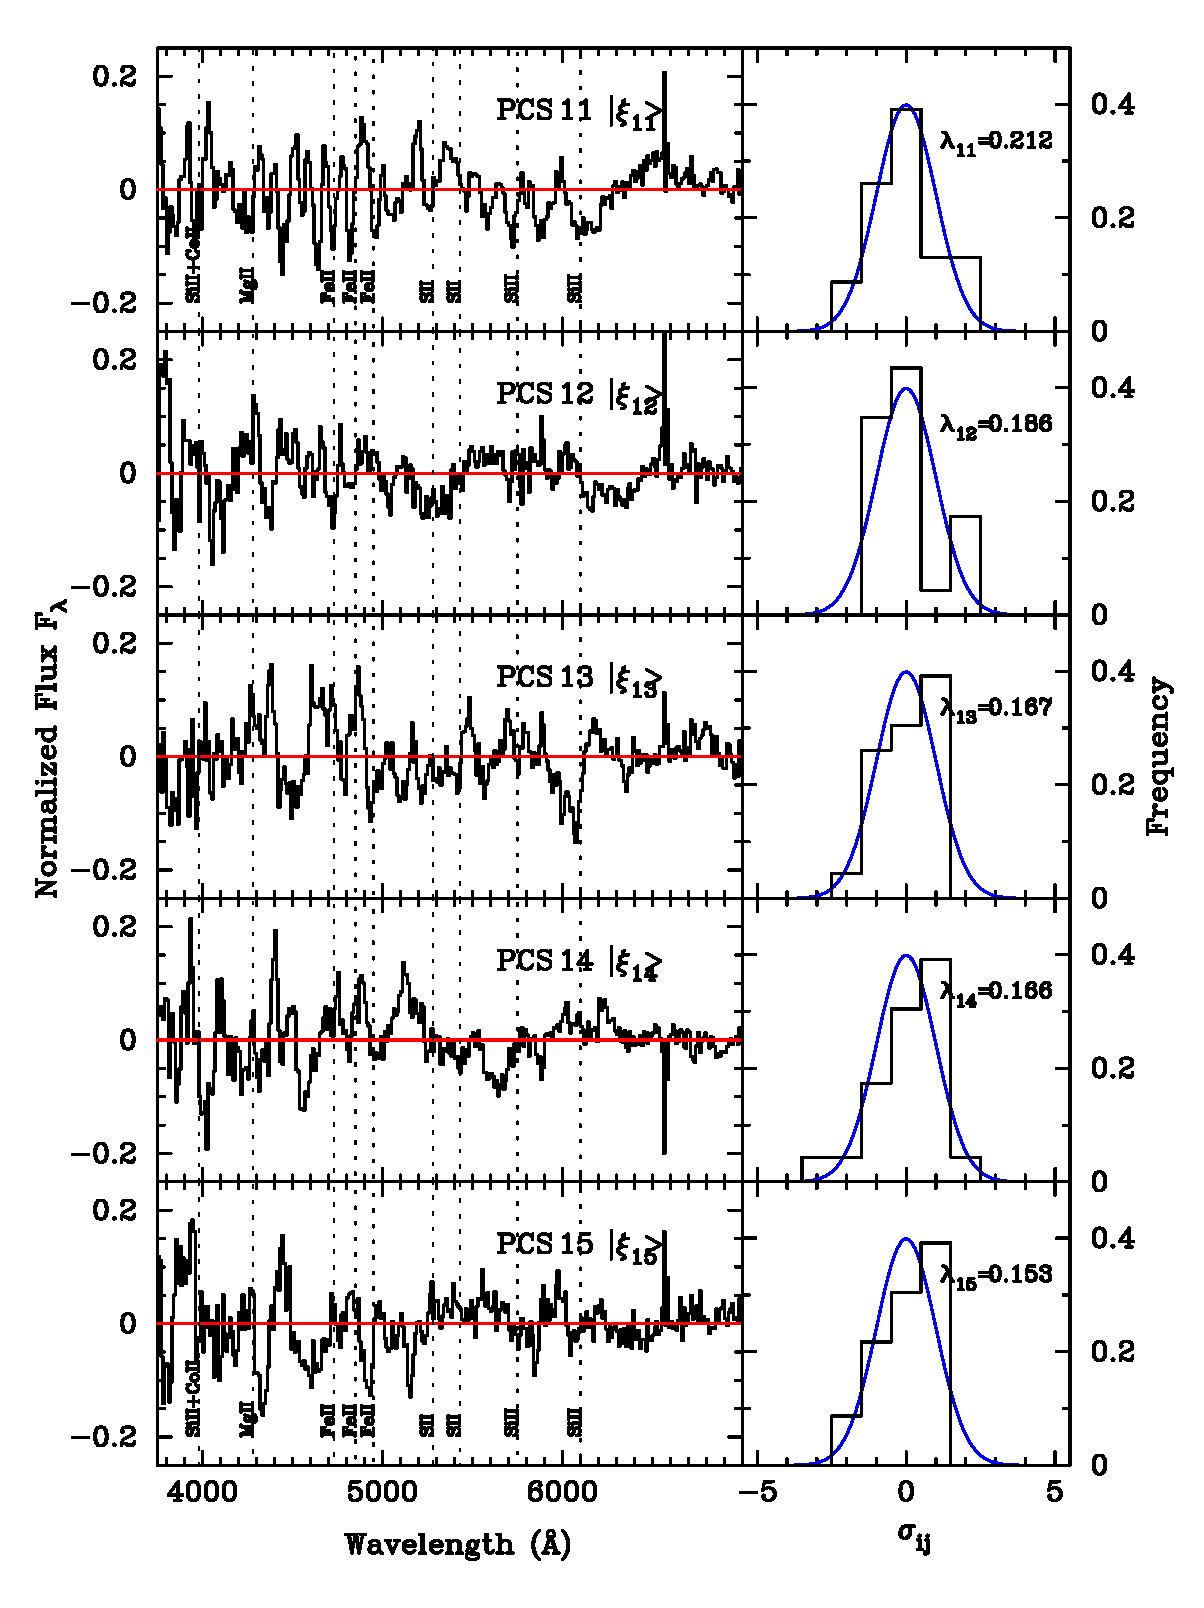
\includegraphics[angle=0,scale=0.8]{./figures/pca/20SNe_PCS_11to15_areanorm.ps}
\end{center}
\caption{
Eigenvectors eleven through fifteen, which account for 0.9\% of variation in the sample. 
}
\label{fig:eigen3}
\end{figure}
\begin{figure}[htp]
\begin{center}
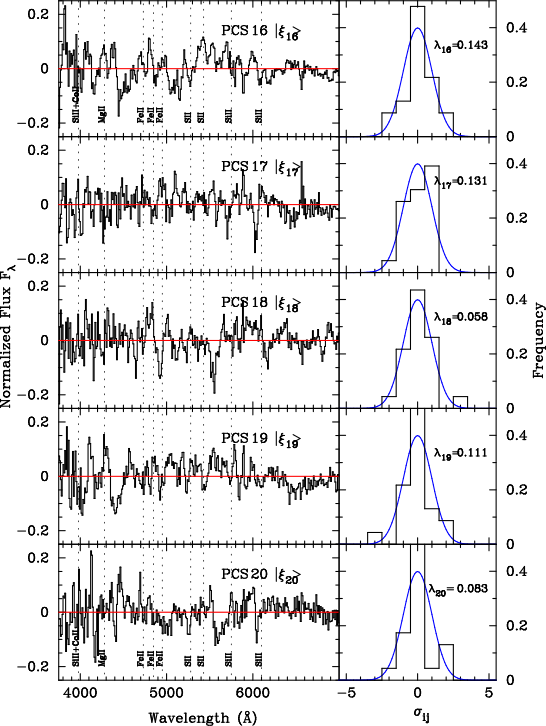
\includegraphics[angle=0,scale=0.8]{./figures/pca/20SNe_PCS_16to20_areanorm.ps}
\end{center}
\caption{
Eigenvectors sixteen through twenty, which account for 0.3\% of variation in the sample. 
}
\label{fig:eigen4}
\end{figure}


\begin{figure}[htp]
\begin{center}
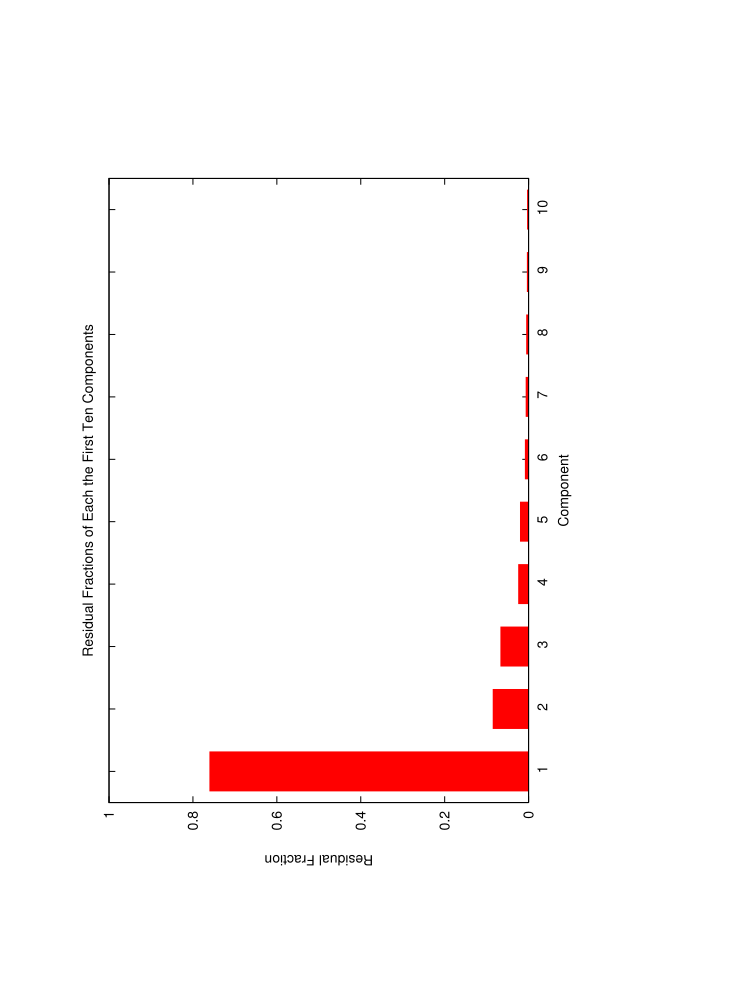
\includegraphics[angle=-90,scale=0.66]{./figures/hand_made/residual_fraction.ps}
\end{center}
\caption{
The residual fraction of the first ten components.
}
\label{fig:residualfrac1-5}
\end{figure}

% Built from SN_residual_fraction.dat
%% The values (usually only l,r and c) in the last part of
%% \begin{deluxetable}{} command tell LaTeX how many columns
%% there are and how to align them.
\begin{deluxetable}{ccccc}

%% Keep a portrait orientation

%% Over-ride the default font size
%% Use Default (12pt)

%% Use \tablewidth{?pt} to over-ride the default table width.
%% If you are unhappy with the default look at the end of the
%% *.log file to see what the default was set at before adjusting
%% this value.

%% This is the title of the table.
\tablecaption{Residual Fractions}

%% This command over-rides LaTeX's natural table count
%% and replaces it with this number.  LaTeX will increment 
%% all other tables after this table based on this number
\tablenum{5}

%% The \tablehead gives provides the column headers.  It
%% is currently set up so that the column labels are on the
%% top line and the units surrounded by ()s are in the 
%% bottom line.  You may add more header information by writing
%% another line between these lines. For each column that requries
%% extra information be sure to include a \colhead{text} command
%% and remember to end any extra lines with \\ and include the 
%% correct number of &s.
\tablehead{\colhead{Component} & \colhead{Eigenvalue} & \colhead{Eigenvalue$^{1/2}$} & \colhead{Fraction} & \colhead{Comulative Fraction} \\ 
\colhead{} & \colhead{$\lambda_{j}^{2}$} & \colhead{$\lambda_{j}$} & \colhead{} & \colhead{} } 

%% All data must appear between the \startdata and \enddata commands
\startdata
1 & 14.2425 & 3.7739 & 0.7606 & 0.7606 \\
2 & 1.6013 & 1.2654 & 0.0855 & 0.8461 \\
3 & 1.2576 & 1.1214 & 0.0672 & 0.9132 \\
4 & 0.4647 & 0.6817 & 0.0248 & 0.9380 \\
5 & 0.3816 & 0.6177 & 0.0204 & 0.9584 \\
6 & 0.1645 & 0.4056 & 0.0088 & 0.9672 \\
7 & 0.1284 & 0.3583 & 0.0069 & 0.9740 \\
8 & 0.1069 & 0.3269 & 0.0057 & 0.9798 \\
9 & 0.0755 & 0.2747 & 0.0040 & 0.9838 \\
10 & 0.0674 & 0.2596 & 0.0036 & 0.9874 \\
11 & 0.0452 & 0.2126 & 0.0024 & 0.9898 \\
12 & 0.0347 & 0.1862 & 0.0019 & 0.9916 \\
13 & 0.0282 & 0.1679 & 0.0015 & 0.9931 \\
14 & 0.0277 & 0.1664 & 0.0015 & 0.9946 \\
15 & 0.0237 & 0.1539 & 0.0013 & 0.9959 \\
16 & 0.0205 & 0.1432 & 0.0011 & 0.9970 \\
17 & 0.0173 & 0.1314 & 0.0009 & 0.9979 \\
18 & 0.0035 & 0.0590 & 0.0002 & 0.9981 \\
19 & 0.0124 & 0.1112 & 0.0007 & 0.9988 \\
20 & 0.0070 & 0.0839 & 0.0004 & 0.9991 \\
21 & 0.0083 & 0.0913 & 0.0004 & 0.9996 \\
22 & 0.0079 & 0.0891 & 0.0004 & 1.0000 \\
\enddata

%% Include any \tablenotetext{key}{text}, \tablerefs{ref list},
%% or \tablecomments{text} between the \enddata and 
%% \end{deluxetable} commands

%% No \tablecomments indicated

%% No \tablerefs indicated

\end{deluxetable}


The first eigenvector alone accounts for 76\% of variation in the data set. While the other eigenvectors are relatively flat, the first eigenvector has a definate slope. This allows it to account for differences in the color of supernovae spectra in the data set, with positive coeffecients creating bluer spectra and negative coefficents creating redder spectra. 

Eigenvectors two through five, which combined account for 19.8\% of variation, are all relatively flat. They primarily control the depths of different lines as well as the ratio of lines.

Eigenvectors six through twenty-two combined account for only 4.2\% of variation in the data set. They primarily appear to represent noise in the spectra, and so do not appear to be useful in classifying or categorizing supernovae.

\subsection{Classification of Supernovae}
$\sigma_{1}$ is primarily responsible for the color of a supernova. Supernova with $\sigma_{1} > 0$ are blue, while those with $\sigma_{1} < 0$ are red. $\sigma_{2}$ and $\sigma_{3}$ control the ratio of various absorption features. We have divided the supernovae into classes based on the values of their $\sigma_{1}$ and $\sigma_{2}$ normalized weights. 

We define a coordinate system such that:

$$ r_{i} = \sqrt( \sigma^{2}_{i1} + \sigma^{2}_{i2} )$$
$$ \tan{\theta_{i}} = \frac {\sigma_{i2}}{\sigma_{i1}} $$

Using this system, classes I-IV are defined by the the four quadrants. We define a class zero centered on the origin with a radius $r_{0}$ defined so that the probability of a supernova lying within it are $P = 0.2$. We solve for $r_{i}$ using:

$$ P(r \le r_{0}) = \int_{0}^{r_{0}} r e^{-r^{2}/2} dr = 1 -  e^{-r_{0}^{2}/2} $$

Class zero supernovae are the 20\% of the sample closest to the mean spectrum. Class I are those supernovae with $\sigma_{1} > 0$ and $\sigma_{2} > 0$. Class I are blue with sharp peaks and deep absorption lines. Class II supernovae are defined by $\sigma_{1} < 0$ and $\sigma_{2} > 0$. The have deep lines, but are red. Class III is defined by $\sigma_{1} > 0$ and $\sigma_{2} < 0$. These supernovae are red, with a spectrum that is more flat with less defined features. SN1991bg is a Class III supernova, nearly two standard deviations from the mean in both of its normalized weights. Class IV are those supernovae with $\sigma_{1} > 0$ and $\sigma_{2} < 0$. They are blue with less pronounced features. SN1991T is a Class IV supernova.

In order to visualize how $\sigma_{1}$ and $\sigma_{2}$ effect the shape of a type Ia spectrum, we have provided a plot of the mean spectrum (figure \ref{fig:classzero}), as well as the mean spectrum plus the first two components set so that we create a spectrum within each class, I through IV (figure \ref{fig:fourclasses}). For each of these four demonstration spectra the weights are one standard deviation from the mean.

\begin{figure}[ht]
\begin{center}
\includegraphics[angle=-90,scale=0.66]{./figures/hand_made/avg.ps}
\end{center}
\caption{
The mean spectrum, $\vec{\mu}$. Class zero are the 20\% of supernovae that are closest to this 
}
\label{fig:classzero}
\end{figure}

\begin{figure}[ht]
\begin{center}
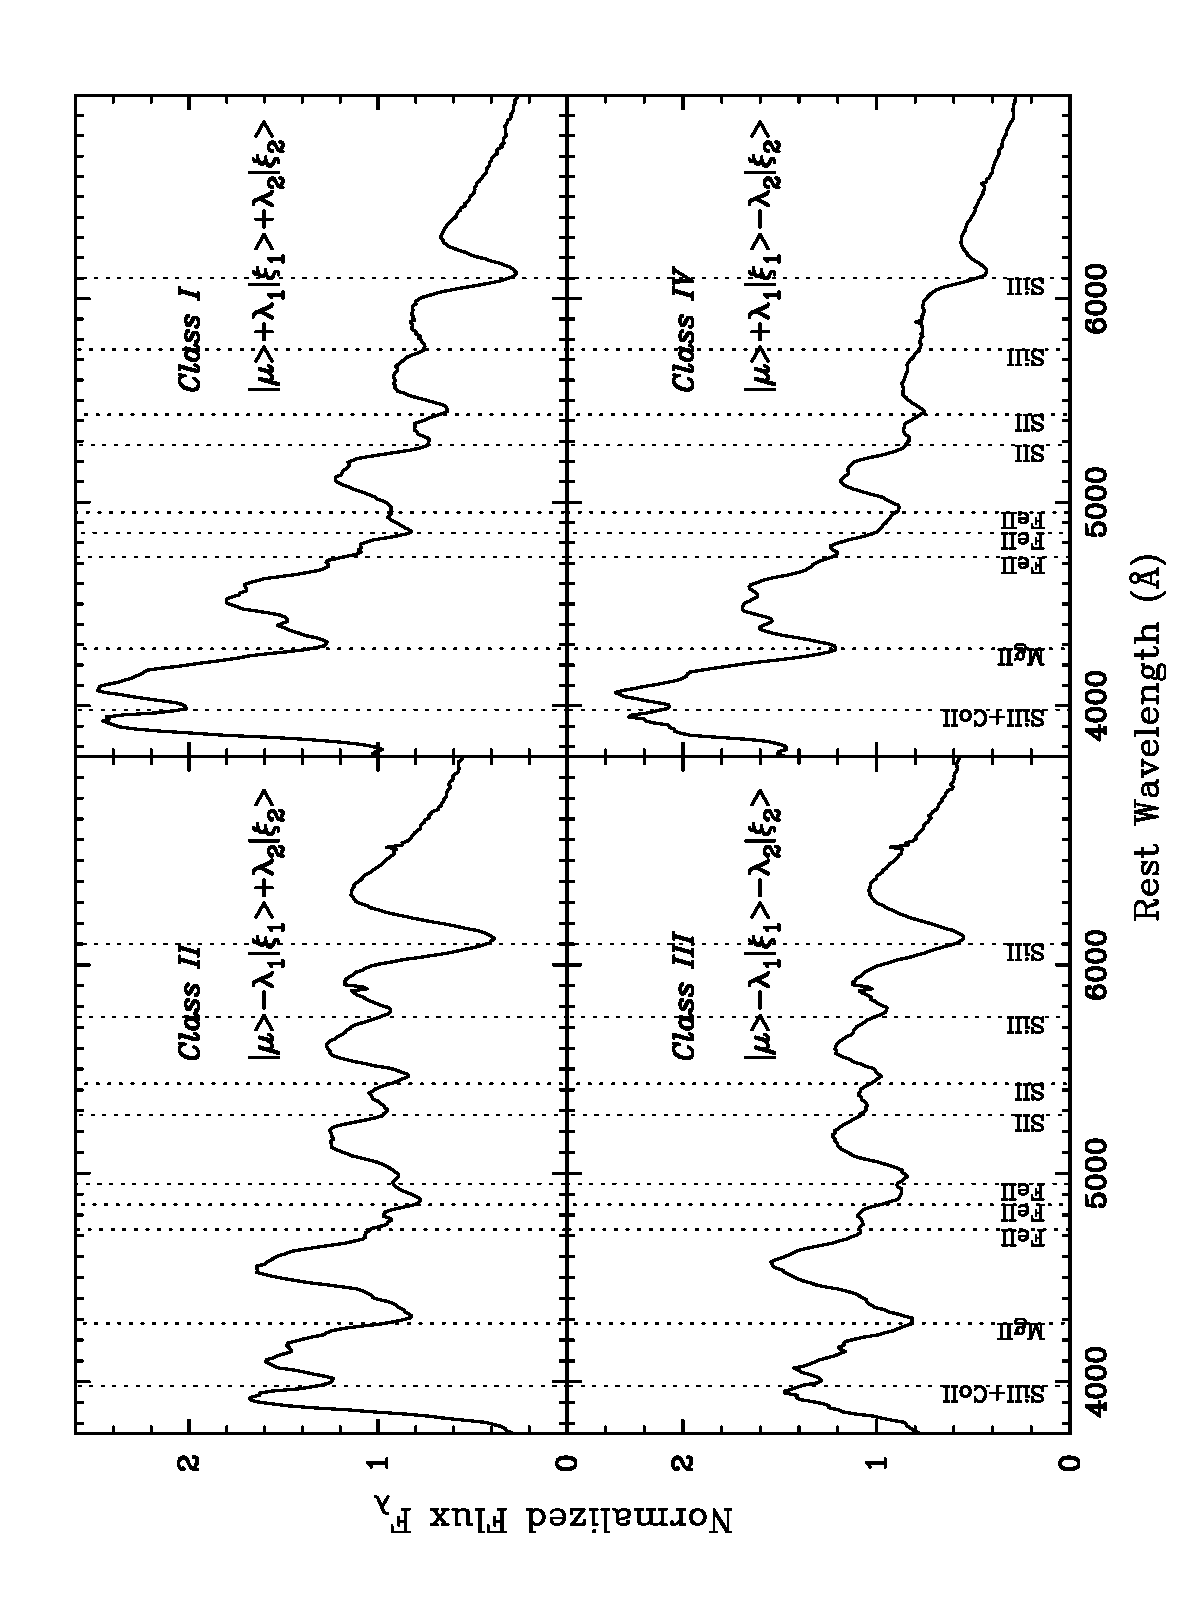
\includegraphics[angle=-90,scale=0.66]{./figures/pca/4class_areanorm.ps}
\end{center}
\caption{
Four spectra demonstrating Class I through Class IV, with the normalized weights set so that each one is one standard deviation from the norm.
}
\label{fig:fourclasses}
\end{figure}

\subsection{Color: Cardelli Law or Intrinsic?}
Although $E(B-V)$ has traditionally been attributed to extinction, recent work has suggested it may not be. For example, recent work by \citeauthor{conley08a} (\citeyear{conley08a}) has indicated that single parameter functions, such as dust laws, are in general unable to reproduce the variation in color seen in supernovae. They further find that the $U - B$ vs. $B - V$ relation found for their type Ia supernovae do not follow the relation one would expect for Milky-Way like dust.

% Conley fig
\begin{figure}[ht]
\begin{center}
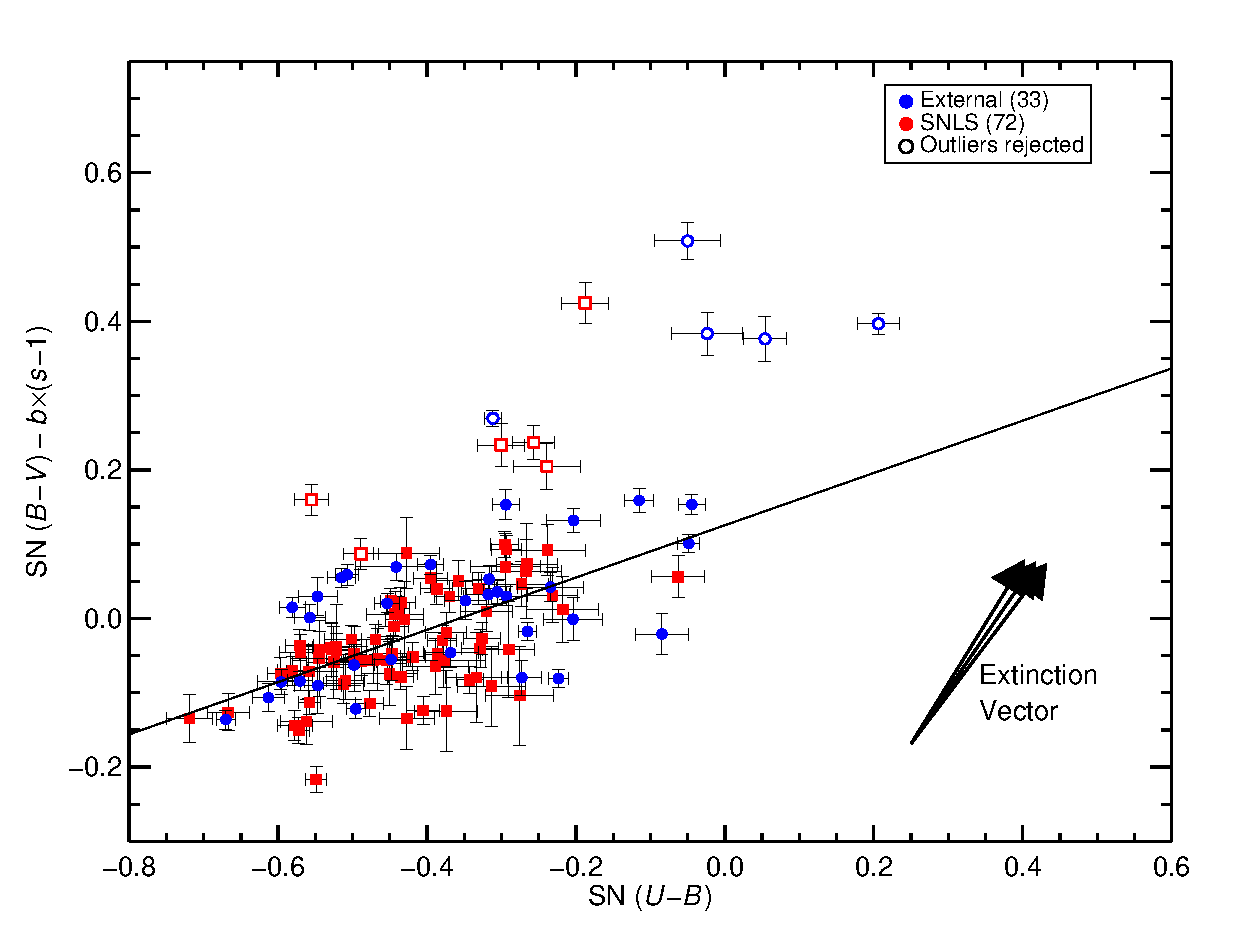
\includegraphics[angle=0,scale=0.8]{./figures/conley/f10_color.eps}
\end{center}
\caption{
The derived $U - B$ vs. $B - V$ relation found by \citeauthor{conley08a} (\citeyear{conley08a}). The best fit to the sample is the solid line. The arrow is the relation one would expect from Milky-Way like dust ($R_{v} = [1.6,3.1,4.6]$). Figure courtesy of \citeauthor{conley08a} (\citeyear{conley08a}).
}
\label{fig:conleyfigure}
\end{figure}

In line with the results of \citeauthor{conley08a} the first eigenvector suggests that color is partially an intrinsic quantity, and not simply due to extinction. If color is purely an extinction related-effect we would expect this eigenvector to be nearly featureless so that line ratios would be completely uncorrelated with color. However, we observe deviations from the first eigenvector that align with the MgII feature, the FeIII features and the SiII features. This suggests that color is, to some extent, correlated with spectral features and is therefore not entirely extinction but is intrinsic to each individual supernova. 

If the color excess observed in type Ia spectra was purely due to extinction then we should be able to use the Cardelli law \citep{cardelli89a} to account for it. We therefore attempt to warp the Hsiao template \citep{hsiao07a}, a template created by taking the mean spectra of over 100 type Ia supernovae near maximum light, with the Cardelli law. We fix $ R_{V} =3.1$ and vary $A_{V}$ until we find a minimum in the $\chi^{2}$ overlap between the warped Hsiao spectrum and the observed spectrum.

While many of the spectra appear to be able to be fit by a simple Cardelli law applied to the Hsiao template, nine supernovae fail. As expected the peculiar SN1991T and SN1991bg are not well fit. SN1998de, SN1998bp, SN1999cl, SN2000dk, and SN2000cx have spectral features that can not be matched with only a Cardelli law. SN1998aq and SN1999aa seem to fit well at first glance, but both have nonphysical preferred values of $A_{V}$, $-0.031$ for SN1998aq and $-0.062$ for SN1999aa. This suggests that for some of the supernovae Cardelli's law does not account for the observed color if $ R_{V} =3.1$ is fixed, however we can not say anything about the effects of letting $R_{V}$ float. This is something that we would like to explore in future work.

<<<<<<< .mine
<<<<<<< .mine
<<<<<<< .mine
<<<<<<< .mine
%%% The values (usually only l,r and c) in the last part of
%% \begin{deluxetable}{} command tell LaTeX how many columns
%% there are and how to align them.
\begin{deluxetable}{cc}

%% Keep a portrait orientation

%% Over-ride the default font size
%% Use Default (12pt)

%% Use \tablewidth{?pt} to over-ride the default table width.
%% If you are unhappy with the default look at the end of the
%% *.log file to see what the default was set at before adjusting
%% this value.

%% This is the title of the table.
\tablecaption{Result Of Warping Hsiao Template With Cardelli Law}

%% This command over-rides LaTeX's natural table count
%% and replaces it with this number.  LaTeX will increment
%% all other tables after this table based on this number
\tablenum{4}

%% The \tablehead gives provides the column headers.  It
%% is currently set up so that the column labels are on the
%% top line and the units surrounded by ()s are in the
%% bottom line.  You may add more header information by writing
%% another line between these lines. For each column that requries
%% extra information be sure to include a \colhead{text} command
%% and remember to end any extra lines with \\ and include the
%% correct number of &s.
\tablehead{\colhead{Well fit supernovae} & \colhead{Badly fit supernovae} \\
\colhead{} & \colhead{} } % for units

%% All data must appear between the \startdata and \enddata commands
\startdata
SN1997dt & SN1991T \\
SN1998aq & SN1991bg \\
SN1999dh & SN1998bp \\
SN1998V  & SN1998de \\
SN1998eg & 
SN1998ec & SN1999ac \\
SN1999aa & SN1999cc \\
SN1999dq & SN1999cl \\
SN1999gd & SN1999ej \\
SN1999gp & SN2000cx \\
SN2000cf & SN2000dk \\
SN2000fa \\
SN2000es
\enddata

%% Include any \tablenotetext{key}{text}, \tablerefs{ref list},
%% or \tablecomments{text} between the \enddata and
%% \end{deluxetable} commands

%% No \tablecomments indicated

%% No \tablerefs indicated

\end{deluxetable}


=======
Warping Hsiao's template with a Cardelli law provides a qualitative indication that color is not entirely due to extinction, but does not provide us with a quantitative method of determining the ammount of color excess due to extinction. For this we turn to our eigenvectors.
=======
Warping Hsiao's template with a Cardelli law provides a qualitative indication that color is not entirely due to extinction, but does not provide us with a quantitative method of determining the amount of color excess due to extinction. For this we turn to our eigenvectors.
=======
Warping Hsiao's template with a Cardelli law provides a qualitative indication that color is not entirely due to extinction, but it does not provide us with a quantitative method of determining the amount of color excess due to extinction. For this we turn to our eigenvectors.
=======
Warping Hsiao's template with a Cardelli law provides a qualitative indication that color is not entirely due to extinction, but it does not provide us with a quantitative method of determining the amount of color excess due to extinction. For this we turn to the eigenvectors.
>>>>>>> .r1177
>>>>>>> .r1139
>>>>>>> .r1130
>>>>>>> .r1097

In figures \ref{fig:sig1sig2}, \ref{fig:sig1sig3}, and \ref{fig:sig2sig3} we plot the normalized weight functions of the supernovae against each other. Supernovae with similar features will cluster. Further, it is possible to calculate a extinction vector in this space which allows us to observe exactly how much color excess is due to extinction. We plot the extinction vector by using the Cardelli law to warp the mean spectrum from the PCA. We fix $R_{V} = 3.1$ and increment $A_{V}$ by 0.2. We then normalize this spectrum by its area again and subtract off the mean spectrum. We then dot this with an eigenvector which gives us a weight. Mathematically this is:

$$ c_{j}^{CCM} = \vec{\xi_{j}} \cdot \left[ \frac {\vec{\mu} \cdot CCM(R_{V}=3.1,A_{V})}{Normalization} - \vec{\mu} \right] $$

Where $\vec{\mu}$ is the mean spectrum, $CCM(R_{V}=3.1,A_{V})$ is the Cardelli factor, and $\vec{\xi_{j}}$ is the $j$th eigenvector.

\begin{figure}[ht]
\begin{center}
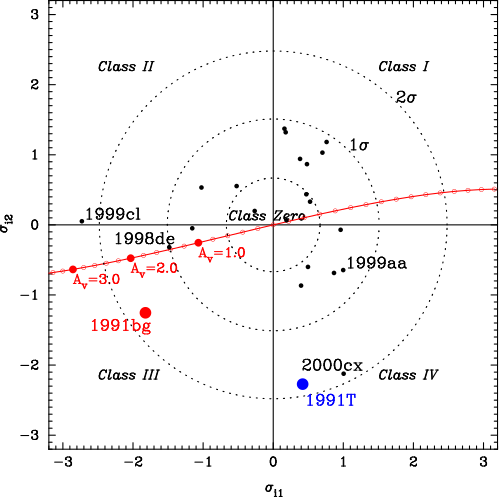
\includegraphics[angle=0,scale=0.8]{./figures/pca/sigma1_vs_sigma2_areanorm.ps}
\end{center}
\caption{
Supernovae plotted by their first and second normalized weight. Supernovae with $\sigma_{1} > 0$ are blue, while those with $\sigma_{1} < 0$ are red. The red line marks the expected extinction vector for Cardelli law extinction, with each open circle marking a step in $A_{V}$ of $0.2$.
}
\label{fig:sig1sig2}
\end{figure}

\begin{figure}[ht]
\begin{center}
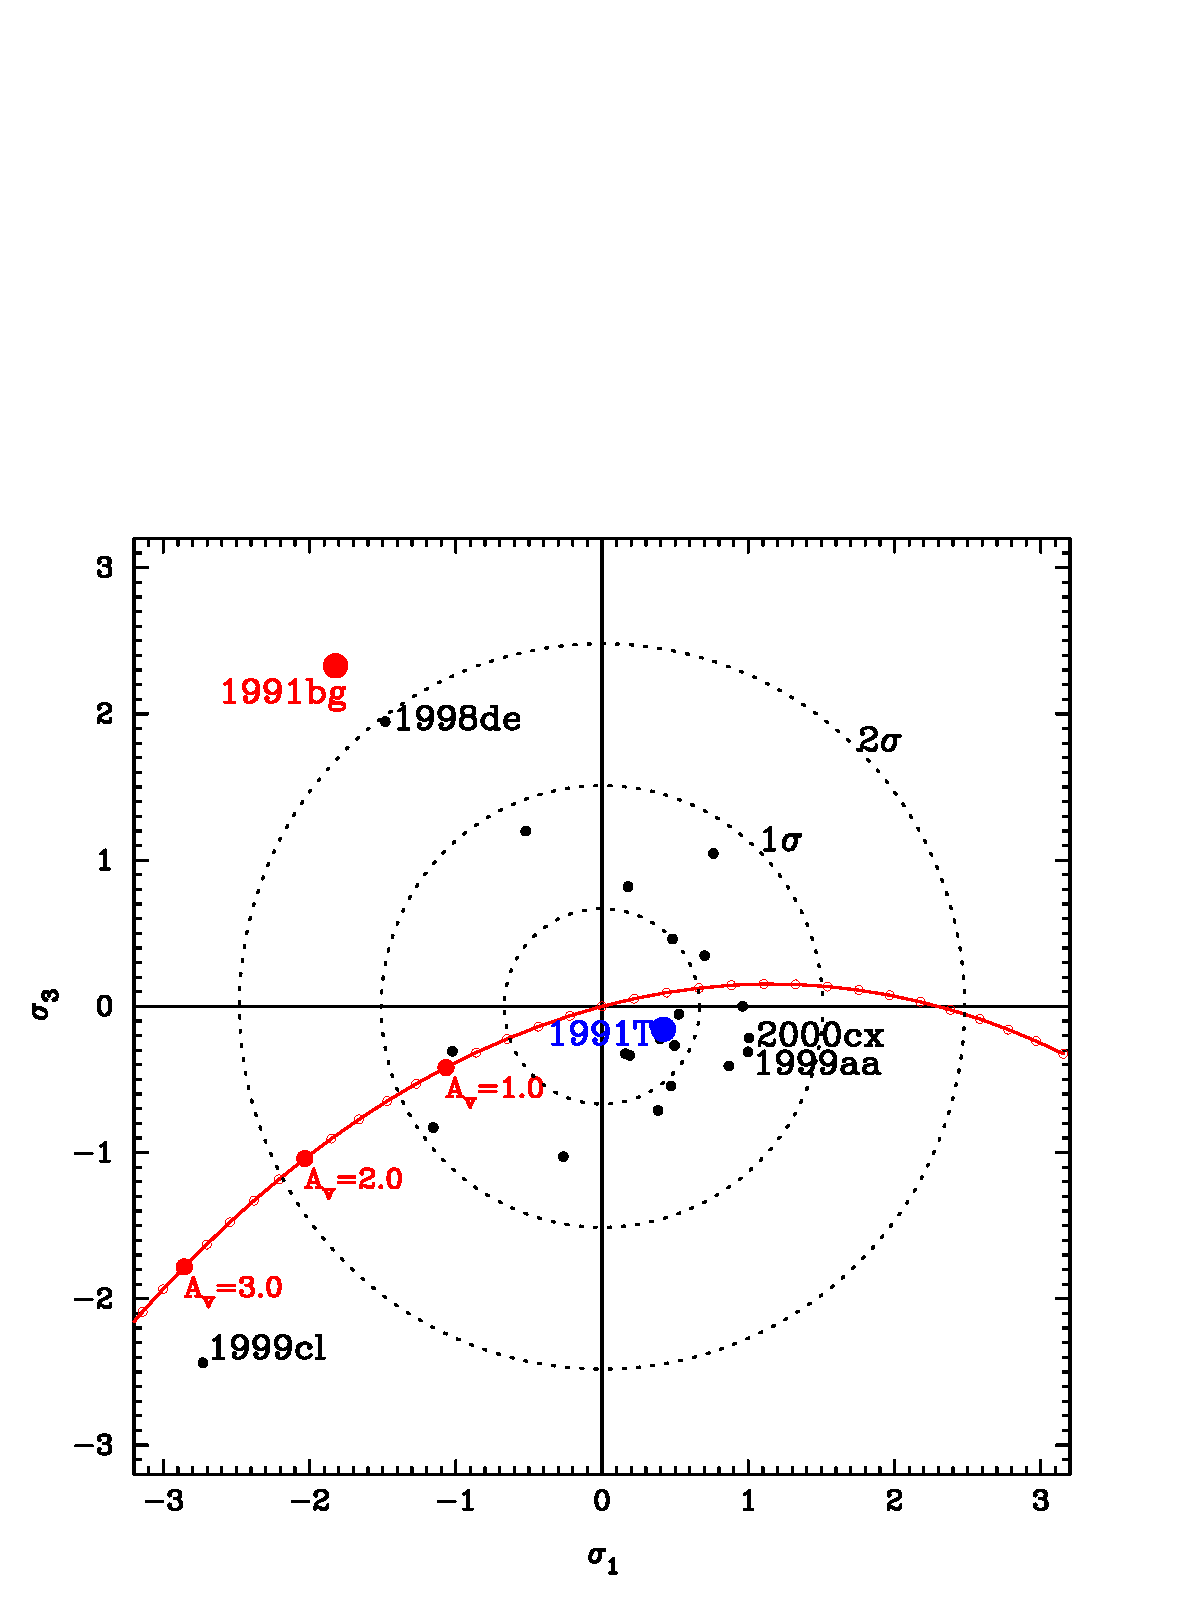
\includegraphics[angle=0,scale=0.8]{./figures/pca/sigma1_vs_sigma3_areanorm.ps}
\end{center}
\caption{
Supernovae plotted by their first and third normalized weight. Supernovae with $\sigma_{1} > 0$ are blue, while those with $\sigma_{1} < 0$ are red. The red line marks the expected extinction vector for Cardelli law extinction, with each open circle marking a step in $A_{V}$ of $0.2$.
}
\label{fig:sig1sig3}
\end{figure}

\begin{figure}[ht]
\begin{center}
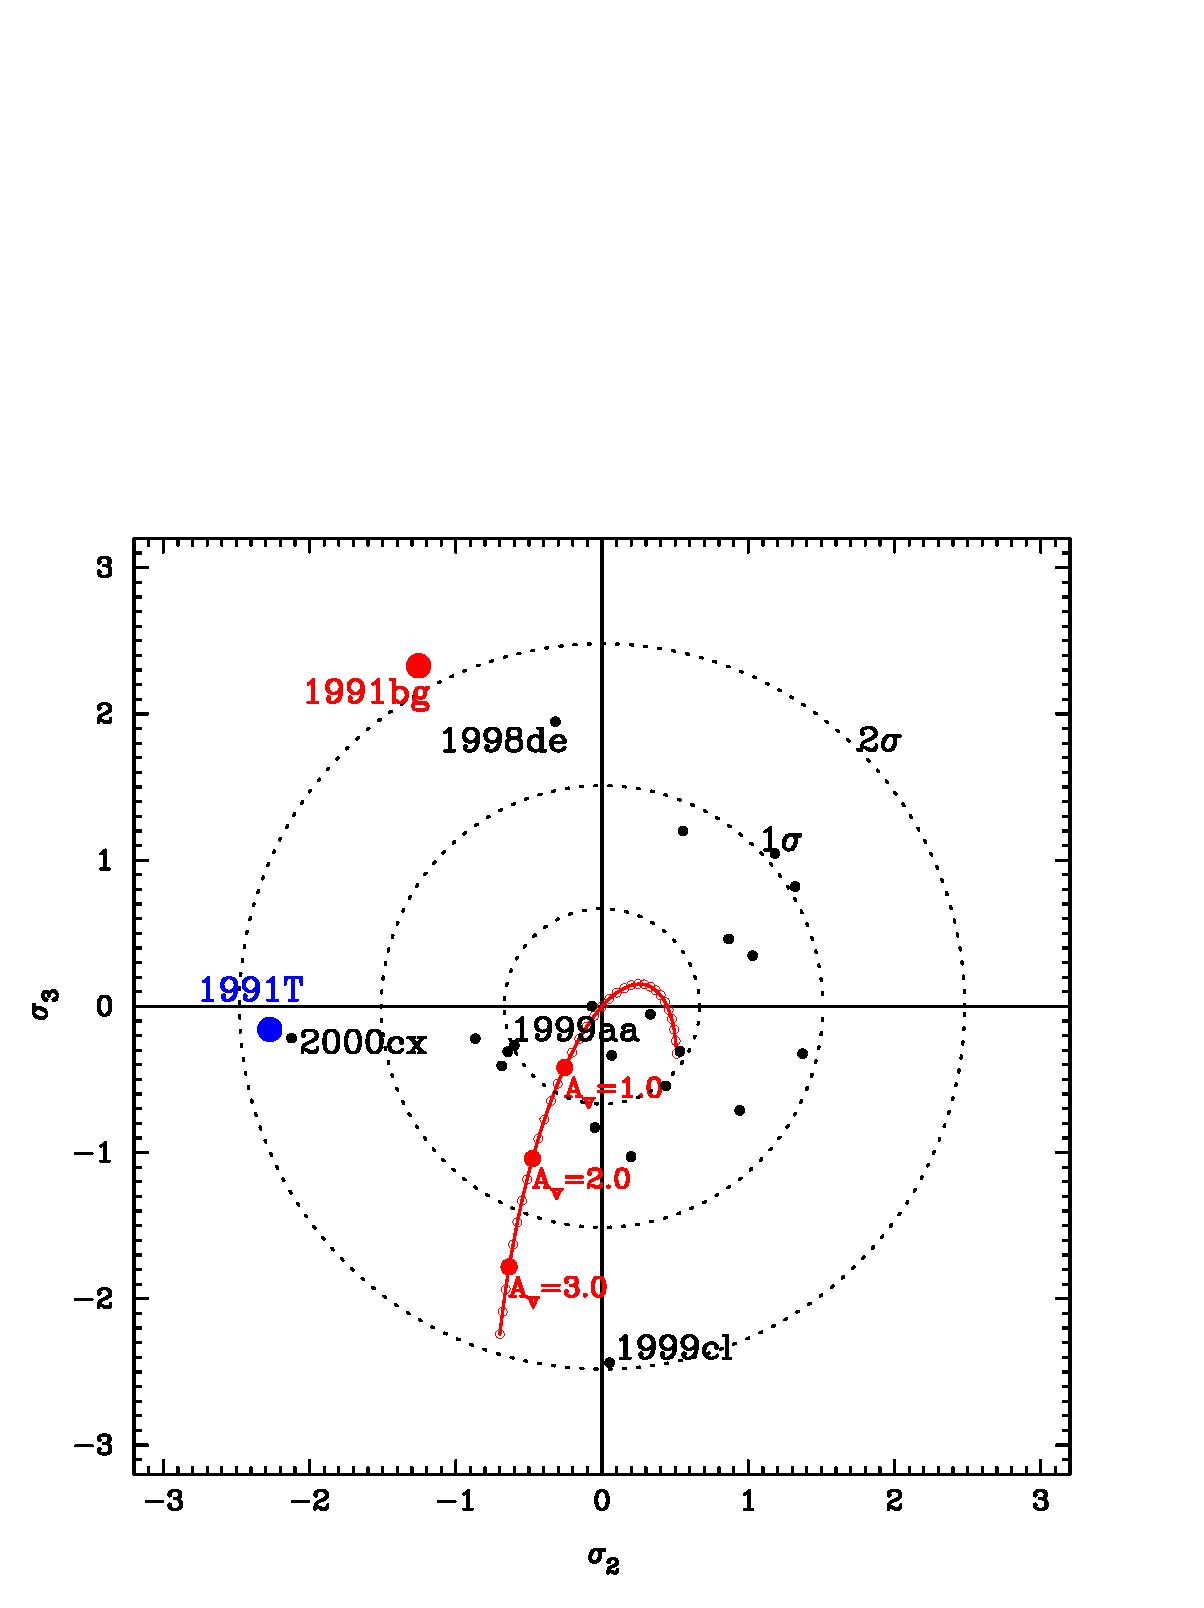
\includegraphics[angle=0,scale=0.8]{./figures/pca/sigma2_vs_sigma3_areanorm.ps}
\end{center}
\caption{
Supernovae plotted by their second and third normalized weight. The red line marks the expected extinction vector for Cardelli law extinction, with each open circle marking a step in $A_{V}$ of $0.2$.
}
\label{fig:sig2sig3}
\end{figure}

Only if a supernova lies near the extinction line, in all three plots, is its color due to Cardelli like dust. It is worth nothing that very few supernovae lie close to the extinction vector in all three plots. This suggests that the variation we see in color from most type Ia supernovae is due to intrinsic properties of the supernovae and not extinction.

\clearpage
\subsection{Applications to the Hubble Diagram}
We hope the PCA eigenvectors will assist in future cosmology research involving type Ia supernovae. In order to get an idea of their usefulness, we create a series of Hubble diagrams with the supernovae from the data set, except for SN1991T and SN1991T as they do not have light curves and SN1999cl which was such an outlier that it badly pulled the fit. We plot $cz$ of the host galaxies of each of the supernovae against their maximum B band magnitude. Because the supernovae are nearby, they have peculiar velocity that must be corrected for. We used the $cz$ calculated relative to the cosmic microwave background \citep{fixsen96a}. We plot the Hubble law using $H_{0} = 71.9 km/s/Mpc$ as reported by \citet{hinshaw08a}.

We also make Hubble diagrams using color corrections (\citeauthor{astier06a} \citeyear{astier06a}; \citeauthor{sullivan03a} \citeyear{sullivan03a}), stretch corrections (\citeauthor{perlmutter97a} \citeyear{perlmutter97a}; \citeauthor{perlmutter99a} \citeyear{perlmutter99a}; \citeauthor{knop03} \citeyear{knop03}), and both color and stretch corrections combined. For these corrections we fit for $\alpha$ and $\beta$ iteratively, seeding with values of $\alpha = -1.24$ and $\beta = 2.28$ as determined by \citet{kowalski08a}. We find that for this sample, $\alpha = -2.084$ and $\beta = 3.610$. In order to find a fit that would correct most of our supernova, we removed by hand a single outlier with color $> 1$.

We then attempt to find a correlation between the normalized weights and dispersion around the Hubble line. While we'd like to be able to measure the effect on intrinsic dispersion, we do not have accurate enough error bars to do so. We plot the first normalized weight, $\sigma_{1}$ against $mag_{B} - Model$ and fit for a correction using weighted least squares. We then apply this correction and plot $\sigma_{2}$ against $mag_{B} - Model - A_{1}*\sigma_{1} - B_{1}$ where $A_{1}$ and $B_{1}$ are the slope and intercept of the correction. We continue to do this for the first five normalized weights. We then create Hubble diagrams using only the $\sigma_{1}$ correction, using $\sigma_{1}$ and $\sigma_{2}$, and so on until we use all of the corrections up to $\sigma_{5}$.

We then attempt to combine color, stretch, and the normalized weights into one correction. We use the same method as before, except we start by plotting $\sigma_{1}$ against $mag_{B} - Model - \alpha (S - 1) - \beta C$ which is the magnitudes already corrected with color and stretch. We repeat the above process, subtracting off corrections for each normalized weight found previously, before fitting a new correction for the next normalized weight.

We now have fourteen Hubble diagrams. Four were made with the uncorrected data, with color corrections, with stretch corrections, and with color and stretch corrections. Five were made with just using the normalized weights, and five were made combing color, stretch, and then using the normalized weights. For each of these Hubble Diagrams we calculate the dispersion, and then use this dispersion to remove any supernovae that are more than two standard deviations from the Hubble line, what we call a 2$\sigma$-cut dispersion. The supernova cut are marked by an $^{*}$ on table 6.

While table 6 seems to indicate that without using the 2$\sigma$-cut, we are able to achieve a lower dispersion with just our first weight than with color, stretch, or color and stretch combined corrections, this is without outlier rejection. If we reject SN1999cl, a four $\sigma$ outlier, and then perform the analysis, we find that the weight correction only improves the dispersion more than color alone, while stretch corrections and color with stretch corrections combined improve it more than using on the first weight. Using more than just the first weight increases dispersion, which is unexpected as PCA is guaranteed to lower dispersion. We see this increased dispersion though because we do not use the exact corrections determined by the PCA, but used a shortcut of fit for the corrections (the $A_{1}$ and $B_{1}$ mentioned above). Future analysis will be done with the PCA determined corrections.

If we apply the 2$\sigma$-cut after rejecting SN1999cl, we find that only using the first normalized weight gets us a dispersion that is lower than using a color correction alone or a stretch correction alone, but is worse than using a stretch correction and color correction combined. Again using more than just the first normalized weight increases the dispersion. Using color, stretch, and the first normalized weight increases dispersion as compared to using just color and stretch alone.

\clearpage
\begin{deluxetable}{ccccccccc}
\tablecaption{Distance From The Hubble Line In Magnitudes}
\tablenum{6}
\tablehead{\colhead{Supernova} & \colhead{Uncorrected} & \colhead{C} & \colhead{S} & \colhead{CS} & \colhead{W1}  & \colhead{W2} & \colhead{W3} & \colhead{CSW1}}
\startdata
SN1997dt & 2.734$^{*}$ & 2.537$^{*}$ & 0.716 & 0.519 & 1.169$^{*}$ & 0.487 & -0.062 & 1.185$^{*}$ \\
SN1998V & 0.074 & 0.010 & -0.054 & -0.118 & -0.294 & -1.130$^{*}$ & -1.446$^{*}$ & -0.217 \\
SN1998aq & 0.286 & 0.123 & 0.732 & 0.569 & 0.227 & -0.448 & -0.747 & 0.272 \\
SN1998bp & 1.503 & 0.962 & 0.530 & -0.012 & 0.389 & -0.536 & -0.476 & 0.367 \\
SN1998de & 2.678$^{*}$ & 2.275$^{*}$ & 0.535 & 0.132 & 0.880 & 0.305 & 0.590 & 0.947 \\
SN1998dh & 0.628 & 0.414 & 0.158 & -0.055 & -0.001 & -1.256$^{*}$ & -1.653$^{*}$ & 0.013 \\
SN1998ec & 0.741 & 0.700 & 0.111 & 0.070 & -0.190 & -0.973 & -1.581$^{*}$ & 0.331 \\
SN1998eg & 0.424 & 0.236 & 0.282 & 0.094 & 0.180 & -0.937 & -1.133 & -0.084 \\
SN1998es & 0.093 & 0.191 & -0.154 & -0.055 & -0.297 & -0.758 & -1.139 & -0.140 \\
SN1999aa & -0.022 & 0.074 & 0.119 & 0.215 & -0.054 & -0.497 & -0.890 & -0.099 \\
SN1999ac & 0.374 & 0.351 & -0.030 & -0.054 & -0.027 & -1.078 & -1.239 & -0.132 \\
SN1999cc & 0.484 & 0.098 & 0.328 & -0.058 & 0.013 & -1.068 & -1.581$^{*}$ & -0.092 \\
SN1999cl & 1.339 & 1.161 & -2.992$^{*}$ & -3.169$^{*}$ & -1.346$^{*}$ & -2.069$^{*}$ & -3.100$^{*}$ & -1.787$^{*}$ \\
SN1999dq & -0.071 & 0.044 & -0.493 & -0.378 & -0.530 & -0.884 & -1.251 & -0.418 \\
SN1999ej & 0.964 & 0.610 & 0.826 & 0.473 & 0.356 & -0.373 & -0.773 & 0.527 \\
SN1999gd & 1.638$^{*}$ & 1.506$^{*}$ & -0.058 & -0.190 & 0.168 & -0.749 & -1.141 & 0.416 \\
SN1999gp & 0.134 & 0.475 & -0.088 & 0.252 & 0.009 & -0.418 & -0.840 & -0.001 \\
SN2000cf & 0.381 & 0.208 & 0.346 & 0.173 & 0.180 & -0.998 & -0.984 & -0.033 \\
SN2000cx & 0.077 & -0.269 & 0.321 & -0.026 & 0.049 & 0.201 & -0.164 & -0.342 \\
SN2000dk & 0.471 & -0.017 & 0.230 & -0.258 & -0.145 & -1.379$^{*}$ & -1.433$^{*}$ & -0.198 \\
SN2000fa & 0.307 & 0.236 & 0.031 & -0.041 & -0.100 & -0.978 & -1.441$^{*}$ & -0.114 \\
\hline
Dispersion & 0.779 & 0.709 & 0.737 & 0.711 & 0.471 & 0.562 & 0.697 & 0.552 \\
2$\sigma$-cut & 0.419 & 0.341 & 0.319 & 0.237 & 0.291 & 0.464 & 0.497 & 0.322 \\
\enddata
\tablecomments{ C has been color corrected, S has been stretch corrected, CS has been color and stretch corrected, W1 has had a correction from the first normalized weight, W2 uses a correction from the first and second normalized weights, W3 uses a correction from the first, second, and third normalized weights. CSW1 uses a color and stretch correction, as well as corrections from the first normalized weight. The Dispersion is calculated as the standard deviation of the entries. 2$\sigma$-cut is the dispersion recalculated with supernovae that are more than two standard deviations from the Hubble line dropped. Entries marked with a $^{*}$ were dropped for the 2$\sigma$-cut calculation.}
\end{deluxetable}

\clearpage
\begin{deluxetable}{ccccccccc}
\tablecaption{Distance From The Hubble Line In Magnitudes}
\tablenum{7}
\tablehead{\colhead{Supernova} & \colhead{Uncorrected} & \colhead{C} & \colhead{S} & \colhead{CS} & \colhead{W1}  & \colhead{W2} & \colhead{W3} &\colhead{CSW1}}
\startdata
SN1997dt & 2.734$^{*}$ & 2.537$^{*}$ & 0.716$^{*}$ & 0.519$^{*}$ & 1.169$^{*}$ & 0.487 & -0.062 & 1.185$^{*}$ \\
SN1998V & 0.074 & 0.010 & -0.054 & -0.118 & -0.294 & -1.130$^{*}$ & -1.446$^{*}$ & -0.217 \\
SN1998aq & 0.286 & 0.123 & 0.732$^{*}$ & 0.569$^{*}$ & 0.227 & -0.448 & -0.747 & 0.272 \\
SN1998bp & 1.503 & 0.962 & 0.530 & -0.012 & 0.389 & -0.536 & -0.476 & 0.367 \\
SN1998de & 2.678$^{*}$ & 2.275$^{*}$ & 0.535 & 0.132 & 0.880$^{*}$ & 0.305 & 0.590 & 0.947$^{*}$ \\
SN1998dh & 0.628 & 0.414 & 0.158 & -0.055 & -0.001 & -1.256$^{*}$ & -1.653$^{*}$ & 0.013 \\
SN1998ec & 0.741 & 0.700 & 0.111 & 0.070 & -0.190 & -0.973 & -1.581$^{*}$ & 0.331 \\
SN1998eg & 0.424 & 0.236 & 0.282 & 0.094 & 0.180 & -0.937 & -1.133$^{*}$ & -0.084 \\
SN1998es & 0.093 & 0.191 & -0.154 & -0.055 & -0.297 & -0.758 & -1.139$^{*}$ & -0.140 \\
SN1999aa & -0.022 & 0.074 & 0.119 & 0.215 & -0.054 & -0.497 & -0.890 & -0.099 \\
SN1999ac & 0.374 & 0.351 & -0.030 & -0.054 & -0.027 & -1.078$^{*}$ & -1.239$^{*}$ & -0.132 \\
SN1999cc & 0.484 & 0.098 & 0.328 & -0.058 & 0.013 & -1.068$^{*}$ & -1.581$^{*}$ & -0.092 \\
SN1999dq & -0.071 & 0.044 & -0.493 & -0.378 & -0.530 & -0.884 & -1.251$^{*}$ & -0.418 \\
SN1999ej & 0.964 & 0.610 & 0.826$^{*}$ & 0.473 & 0.356 & -0.373 & -0.773 & 0.527 \\
SN1999gd & 1.638$^{*}$ & 1.506$^{*}$ & -0.058 & -0.190 & 0.168 & -0.749 & -1.141$^{*}$ & 0.416 \\
SN1999gp & 0.134 & 0.475 & -0.088 & 0.252 & 0.009 & -0.418 & -0.840 & -0.001 \\
SN2000cf & 0.381 & 0.208 & 0.346 & 0.173 & 0.180 & -0.998$^{*}$ & -0.984 & -0.033 \\
SN2000cx & 0.077 & -0.269 & 0.321 & -0.026 & 0.049 & 0.201 & -0.164 & -0.342 \\
SN2000dk & 0.471 & -0.017 & 0.230 & -0.258 & -0.145 & -1.379$^{*}$ & -1.433$^{*}$ & -0.198 \\
SN2000fa & 0.307 & 0.236 & 0.031 & -0.041 & -0.100 & -0.978 & -1.441$^{*}$ & -0.114 \\
\hline
Dispersion & 0.785 & 0.713 & 0.319 & 0.237 & 0.371 & 0.493 & 0.551 & 0.396 \\
2$\sigma$-cut & 0.374 & 0.283 & 0.247 & 0.187 & 0.224 & 0.451 & 0.461 & 0.254 \\
\enddata
\tablecomments{ The same as table 6, but SN1999cl has been removed before any calculations.}
\end{deluxetable}

\clearpage

\begin{figure}[ht]
\begin{center}
\includegraphics[angle=-90,scale=0.66]{./figures/hand_made/01_hubble.ps}
\end{center}
\caption{
Hubble diagram of uncorrected supernovae.
}
\label{fig:hduncor}
\end{figure}
\clearpage

\begin{figure}[ht]
\begin{center}
\includegraphics[angle=-90,scale=0.66]{./figures/hand_made/02_hubble_stretch_corrected.ps}
\end{center}
\caption{
Hubble diagram of stretch corrected supernovae.
}
\label{fig:hds}
\end{figure}
\clearpage

\begin{figure}[ht]
\begin{center}
\includegraphics[angle=-90,scale=0.66]{./figures/hand_made/03_hubble_color_corrected.ps}
\end{center}
\caption{
Hubble diagram of color corrected supernovae.
}
\label{fig:hdc}
\end{figure}
\clearpage

\begin{figure}[ht]
\begin{center}
\includegraphics[angle=-90,scale=0.66]{./figures/hand_made/04_hubble_color_stretch_corrected.ps}
\end{center}
\caption{
Hubble diagram of color and stretch corrected supernovae.
}
\label{fig:hdcs}
\end{figure}
\clearpage

\begin{figure}[ht]
\begin{center}
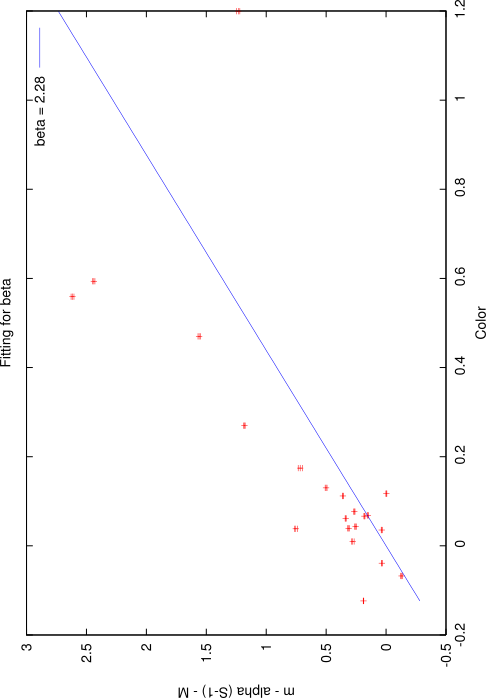
\includegraphics[angle=-90,scale=0.66]{./figures/hand_made/05_hubble_beta.ps}
\end{center}
\caption{
$\beta=3.610$, and the supernovae.
}
\label{fig:beta}
\end{figure}
\clearpage

\begin{figure}[ht]
\begin{center}
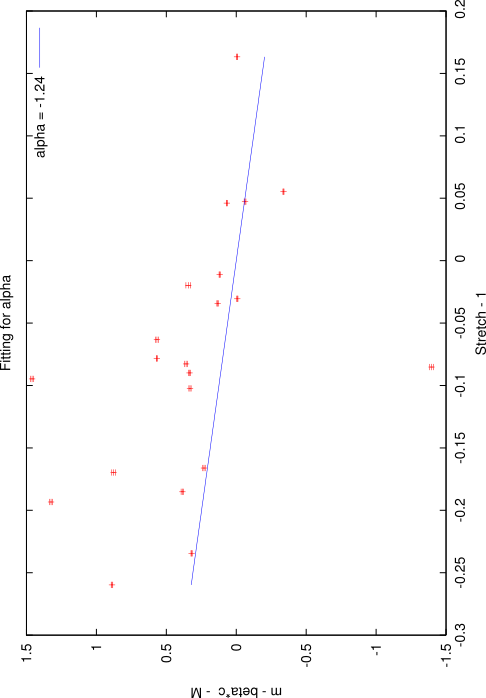
\includegraphics[angle=-90,scale=0.66]{./figures/hand_made/06_hubble_alpha.ps}
\end{center}
\caption{
$\alpha = -2.084$, and the supernovae.
}
\label{fig:alpha}
\end{figure}
\clearpage

\begin{figure}[ht]
\begin{center}
\includegraphics[angle=-90,scale=0.66]{./figures/hand_made/07_hubble_sig_corrected.ps}
\end{center}
\caption{
Hubble diagram of first normalized weight corrected supernovae.
}
\label{fig:hdw}
\end{figure}
\clearpage

\begin{figure}[ht]
\begin{center}
\includegraphics[angle=-90,scale=0.66]{./figures/hand_made/08_hubble_color_stretch_sig_corrected.ps}
\end{center}
\caption{
Hubble diagram of color, stretch, and first normalized weight corrected supernovae.
}
\label{fig:hdcsw}
\end{figure}
\clearpage
